
\cleardoublepage{}

\thispagestyle{empty}
{
    \calccentering{\unitlength}
    \begin{adjustwidth*}{\unitlength}{-\unitlength}
        \raggedleft{}
        {\Huge\color{Burgundy}%
        Exposing Hardware Building Blocks\\
        to Machine Learning Frameworks}\\[\baselineskip]
        {\LARGE%
        Bachelor Thesis}\\[0.1\textheight]
        % \vspace*{\baselineskip}
        {\Huge%[width=0.7\columnwidth]
        Yash Akhauri}\\[\baselineskip]
        {\LARGE%
        01st~December 2019}
        \\[32pt]
        \vfill
        % 
        
\includegraphics[width=70pt]{figures/bison/birla.png} 
        \hfill
        
\includegraphics[width=200pt]{figures/bison/xilinx.jpg}
        \\[32pt]
        \vfill
        % % \begin{wrapfigure}
        % % \centering
        % 
\includegraphics[width=0.4\columnwidth]{figures/bison/birla.png} 
        % % \end{wrapfigure}
            {\large%
            Submitted in partial fulfillment of the requirements\\
            for the degree of Bachelor of Engineering\\[\baselineskip]% (Dr.\ rer.\ nat.)\\[\baselineskip]
    
            to the\\[\baselineskip]
    
            Faculty of Electronics and Instrumentation\\
            at Birla Institute of Technology and Science\\[2\baselineskip]
    
            \begin{minipage}{0.5\textwidth}
            \begin{tabular}{lr}
                1st~~Reviewer & Prof.\ Dr. Surekha Bhanot\\
                2nd Reviewer & Dr.\; Yaman Umuroglu\\
                3rd~~Reviewer & Nicholas Fraser\\
                4th~~Reviewer & Michaela Blott
            \end{tabular}
            \end{minipage}
            \hspace*{36pt}
            %}\hspace*{-8pt}
            %\vspace{2\baselineskip}
            %Datum der Disputation: 13.\ Dezember 2019
            \vfill
            }
            
        % {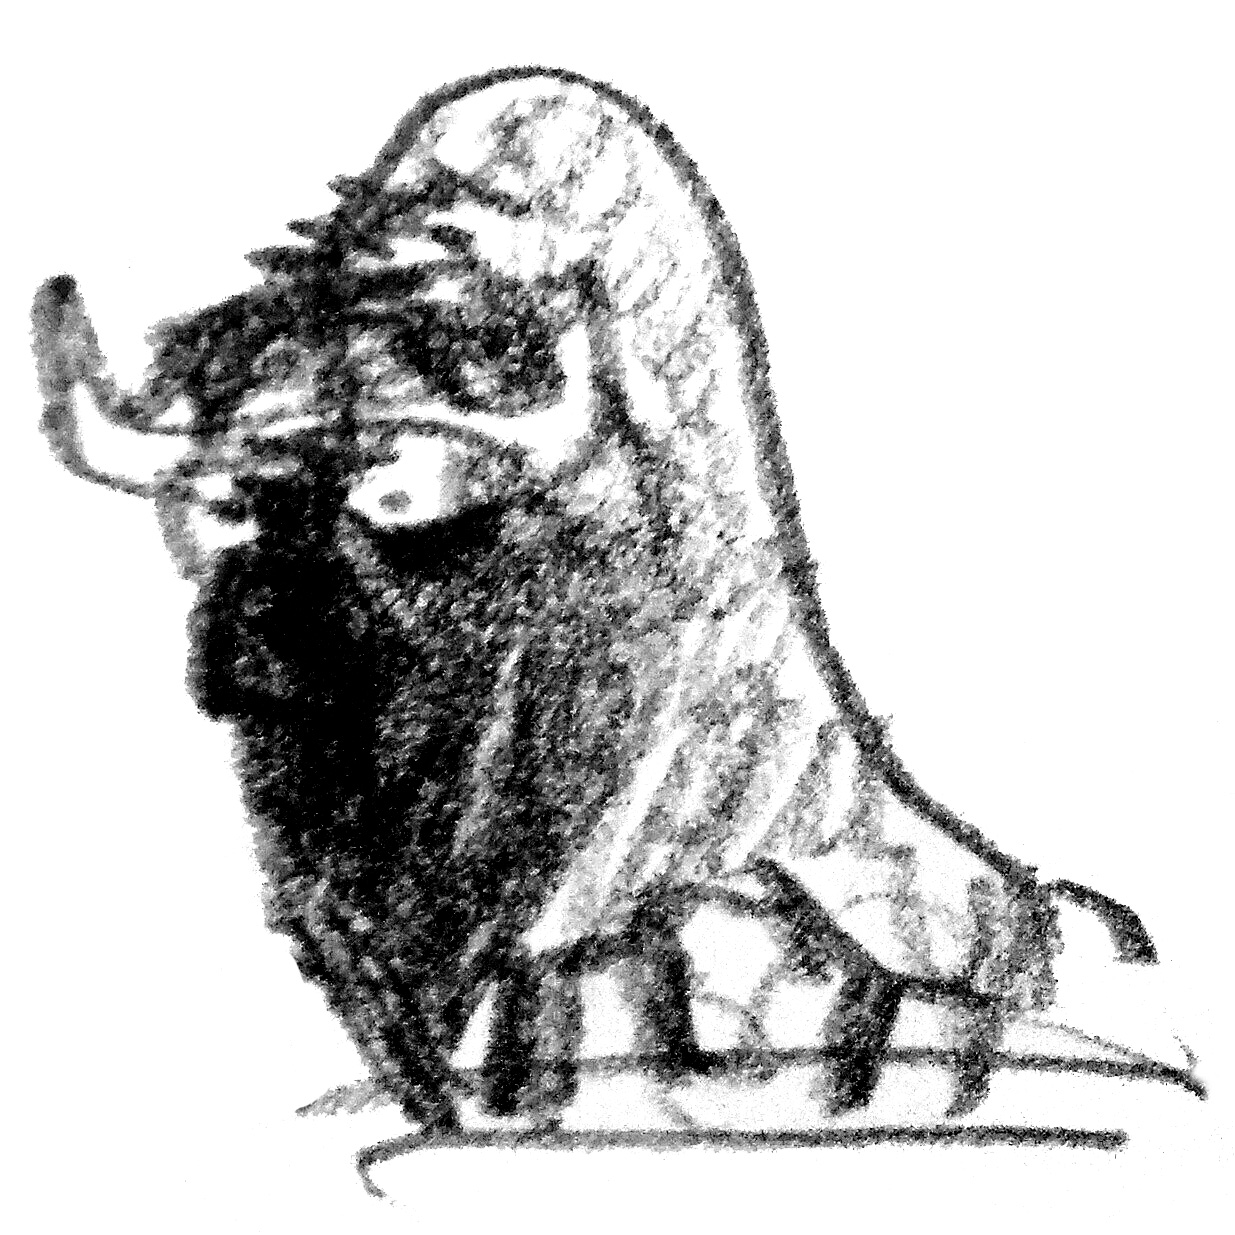
\includegraphics{figures/bison/bison-qed.jpg}}
        \vspace*{\baselineskip}
    \end{adjustwidth*}
}

\clearpage{}

% verso: colophon / impressum
\thispagestyle{empty}
\hphantom{.}
\vfill

\section*{Imprint}

\textit{Exposing Hardware Building Blocks to Machine Learning Frameworks}\\
Copyright \textcopyright{} 2019 by \theauthor{}.\\
All rights reserved. Printed in India.\\
Published by the Birla Institute of Technology and Science.

\section*{Colophon}

This thesis was typeset using \LaTeX{} and the \texttt{memoir} documentclass.
It is based on Aaron Turon's thesis \emph{Understanding and expressing scalable concurrency}\footnote{\url{https://people.mpi-sws.org/~turon/turon-thesis.pdf}}, itself a mixture of \texttt{classicthesis}\footnote{\url{https://bitbucket.org/amiede/classicthesis/}} by Andr\'e Miede and \texttt{tufte-latex}\footnote{\url{https://github.com/Tufte-LaTeX/tufte-latex}}, based on Edward Tufte's \emph{Beautiful Evidence}.\\[0.5\baselineskip]
%
The bibliography was processed by Biblatex.
All graphics and plots are made with PGF/Ti\emph{k}Z.\\[0.5\baselineskip]
%
The body text is set 10/14pt (long primer) on a 26pc measure.
The margin text is set 8/9pt (brevier) on a 12pc measure.
Matthew Carter's \textrm{Charter} acts as both the text and display typeface.
Monospaced text uses Jim Lyles's \texttt{Bitstream Vera Mono} (\enquote{Bera Mono}).

\clearpage{}

% % recto: dedication or epigraph
\thispagestyle{empty}
\vphantom{.}
\vfill
{%
    \flushright{}
    \emph{If we knew what it was we were doing,\\
          it would not be called research, would it?}\\
    \hfill---Albert Einstein
}
\vfill
\vfill

% verso: blank
% \clearpage{}
